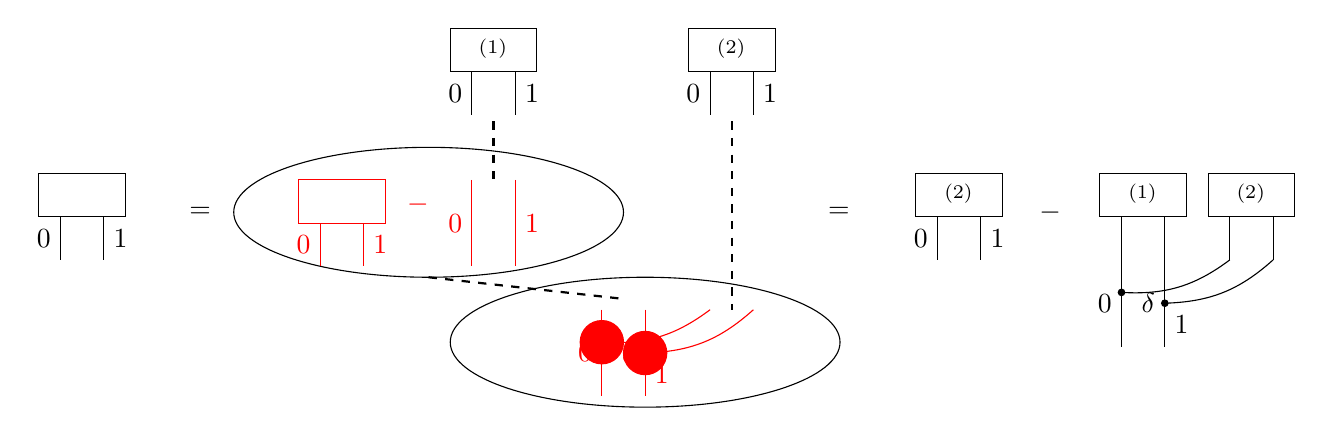
\begin{tikzpicture}[scale=0.275] % , baseline = -3.5pt



\begin{scope}[shift={(-19,-1.7)}]
		%\draw[] (-1,2.2) ellipse (4 and 2.5);
	  	\draw  (-3,2) rectangle (1,4);
		\node at (-1,1.9) [above] {${\exformula}$};
		\draw (-2,2) -- (-2,0) node[midway,left] {$\catvariableof{0}$};
		\draw (0,2) -- (0,0) node[midway,right] {$\catvariableof{1}$};	
		\node at (3.5,2.2)[right]  {$=$};
\end{scope}

\draw[] (-4,0.5) ellipse (9 and 3);
   	\begin{scope}[shift={(-2,-2)}]
  		\draw[\skeletoncolor] (-8,2) rectangle (-4,4);
		\node at (-6,2) [above,\skeletoncolor] {$\ones$};
		\draw[\skeletoncolor] (-7,2) -- (-7,0) node[midway,left] {$\catvariableof{0}$};
		\draw[\skeletoncolor] (-5,2) -- (-5,0) node[midway,right] {$\catvariableof{1}$};
	\end{scope}
	
	\draw[\skeletoncolor] (-2,2) -- (-2,-2) node[midway,left] {$\catvariableof{0}$};
	\draw[\skeletoncolor](0,2) -- (0,-2) node[midway,right] {$\catvariableof{1}$};
	\node[\skeletoncolor] at (-4.5,0) [above] {$-$};
\draw[thick,dashed] (-4,-2.5) -- (5,-3.5);
%\draw[] (6,-2.5) -- (1,-2.5);

%% Into negation core
\draw[thick,dashed] (-1,4.7) -- (-1,2);%-4,3.5);

%% Into conjunction core
\draw[thick,dashed] (10,4.7) -- (10,-4);%(6,-2.5);


\begin{scope}[shift={(10,-6)}]
	\draw[] (-4,0.5) ellipse (9 and 3);
	\begin{scope}[shift={(-4,0)}]
		\renewcommand{\skeletoncolor}{red}
	\node at (0,0) [left,\skeletoncolor] {$\delta$};
	\draw[\skeletoncolor]  (0,2) -- (0,0);% node[midway,left] {$\placeholderof{1}$};
	\draw[fill,\skeletoncolor] (0,0) circle (\dotsize);
	\draw[\skeletoncolor] (0,0) -- (0,-2) node[midway,right] {$\catvariableof{1}$};
	\draw[\skeletoncolor] (5,2) to[bend left=20] (0,0);


	\draw[fill,\skeletoncolor] (-2,0.5) circle (\dotsize);
	\draw[\skeletoncolor] (3,2) to[bend left=20] (-2,0.5);
	\draw[\skeletoncolor] (-2,2) -- (-2,-2) node[midway,left] {$\catvariableof{0}$};
	\end{scope}
\end{scope}



\begin{scope}[shift={(0,5)}]
		%\draw[] (-1,2.2) ellipse (4 and 2.5);
	  	\draw  (-3,2) rectangle (1,4);
		\node at (-1,1.9) [above] {${\secexformula^{(1)}}$};
		\draw (-2,2) -- (-2,0) node[midway,left] {$\catvariableof{0}$};
		\draw (0,2) -- (0,0) node[midway,right] {$\catvariableof{1}$};	
\end{scope}

\begin{scope}[shift={(11,5)}]
		%\draw[] (-1,2.2) ellipse (4 and 2.5);
	  	\draw  (-3,2) rectangle (1,4);
		\node at (-1,1.9) [above] {${\secexformula^{(2)}}$};
		\draw (-2,2) -- (-2,0) node[midway,left] {$\catvariableof{0}$};
		\draw (0,2) -- (0,0) node[midway,right] {$\catvariableof{1}$};	
		
\end{scope}




\node at (14,0.5)[right]  {$=$};


\begin{scope}[shift={(29,0)}]

\begin{scope}[shift={(-7.5,-1.7)}]
		%\draw[] (-1,2.2) ellipse (4 and 2.5);
	  	\draw[]  (-3,2) rectangle (1,4);
		\node at (-1,1.9) [above] {${\secexformula^{(2)}}$};
		\draw[] (-2,2) -- (-2,0) node[midway,left] {$\catvariableof{0}$};
		\draw[] (0,2) -- (0,0) node[midway,right] {$\catvariableof{1}$};	
		\node at (2.25,2.2)[right]  {$-$};		
\end{scope}


\begin{scope}[shift={(1,-3.7)}]
%	\renewcommand{\skeletoncolor}{\conjunctioncolor}
	\node at (0,0) [left] {$\delta$};
	\draw[]  (0,2) -- (0,0);% node[midway,left] {$\placeholderof{1}$};
	\draw[fill] (0,0) circle (0.15cm);
	\draw[] (0,0) -- (0,-2) node[midway,right] {$\catvariableof{1}$};
	\draw[] (5,2) to[bend left=20] (0,0);


	\draw[fill] (-2,0.5) circle (0.15cm);
	\draw[] (3,2) to[bend left=20] (-2,0.5);
	\draw[] (-2,2) -- (-2,-2) node[midway,left] {$\catvariableof{0}$};
\end{scope}


\begin{scope}[shift={(1,-1.7)}]
		%\draw[] (-1,2.2) ellipse (4 and 2.5);
	  	\draw  (-3,2) rectangle (1,4);
		\node at (-1,1.9) [above] {${\secexformula^{(1)}}$};
		\draw[] (-2,2) -- (-2,0); % node[midway,left] {$\catvariableof{0}$};
		\draw[] (0,2) -- (0,0); % node[midway,right] {$\catvariableof{1}$};	
	
\end{scope}
	
\begin{scope}[shift={(6,-1.7)}]
		%\draw[] (-1,2.2) ellipse (4 and 2.5);
	  	\draw[]  (-3,2) rectangle (1,4);
		\node at (-1,1.9) [above] {${\secexformula^{(2)}}$};
		\draw[]  (-2,2) -- (-2,0); % node[midway,left] {$\catvariableof{0}$};
		\draw[]  (0,2) -- (0,0); % node[midway,right] {$\catvariableof{1}$};	
	
\end{scope}

\end{scope}



	
	
\end{tikzpicture}